\documentclass[aspectratio=169, dvipdfmx, 11pt]{beamer}
\usepackage{here, amsmath, latexsym, amssymb, bm, ascmac, mathtools, multicol, tcolorbox, subfig}

% Design
\usetheme{Madrid}
% Color theme
\usecolortheme{orchid}
% Font theme
\usefonttheme{professionalfonts}
% In frame
\useinnertheme{circles}
% Out of frame
\useoutertheme{infolines}
% Garbage cancellation of bookmark
\usepackage{atbegshi}
\ifnum 42146=\euc"A4A2
\AtBeginShipoutFirst{\special{pdf:tounicode EUC-UCS2}}
\else
\AtBeginShipoutFirst{\special{pdf:tounicode 90ms-RKSJ-UCS2}}
\fi
% Hide navigation bar
\setbeamertemplate{navigation symbols}{}
% Make the default gothic
\renewcommand{\kanjifamilydefault}{\gtdefault}
% Title color
\setbeamercolor{title}{fg=structure, bg=}
% Frame title color
\setbeamercolor{frametitle}{fg=structure, bg=}
% Display slide number only
% \setbeamertemplate{footline}[frame number]
% Itemize
\setbeamertemplate{itemize item}{\small\raise0.5pt\hbox{$\bullet$}}
\setbeamertemplate{itemize subitem}{\tiny\raise1.5pt\hbox{$\blacktriangleright$}}
\setbeamertemplate{itemize subsubitem}{\tiny\raise1.5pt\hbox{$\bigstar$}}
% Color
\newcommand{\red}[1]{\textcolor{red}{#1}}
\newcommand{\green}[1]{\textcolor{green!40!black}{#1}}
\newcommand{\blue}[1]{\textcolor{blue!80!black}{#1}}

\title{論文紹介}
\subtitle{Mask R-CNN}
\author{松永 葵}
\institute{谷口研究室 B4}
\date{2019/04/17}

\begin{document}
\maketitle

\begin{frame}{目次}
    \tableofcontents
\end{frame}

\section{はじめに}
\begin{frame}{目次}
    \tableofcontents[currentsection]
\end{frame}

\begin{frame}{物体検出について}
	\begin{itemize}
    	\item 物体検出
        \begin{itemize}
        	\item 物体を矩形領域で抽出 \\
        \end{itemize}
        \item セマンティックセグメンテーション \\
        \begin{itemize}
        	\item ピクセルひとつひとつにラベルを割り当てる \\
            \item ただし、同じラベルの物体が重なっていると、物体同士の境界がわからない \\
        \end{itemize}
        \item インスタンスセグメンテーション \\
        \begin{itemize}
        	\item 物体検出 + セマンティックセグメンテーション \\
			\item それぞれの物体を区別しつつ、物体がある領域をピクセル単位で分類
        \end{itemize}
    \end{itemize}
\end{frame}


\section{Mask R-CNN}
\begin{frame}{目次}
    \tableofcontents[currentsection]
\end{frame}

\begin{frame}{Mask R-CNNとは}
    \begin{figure}[htb]
		\centering
		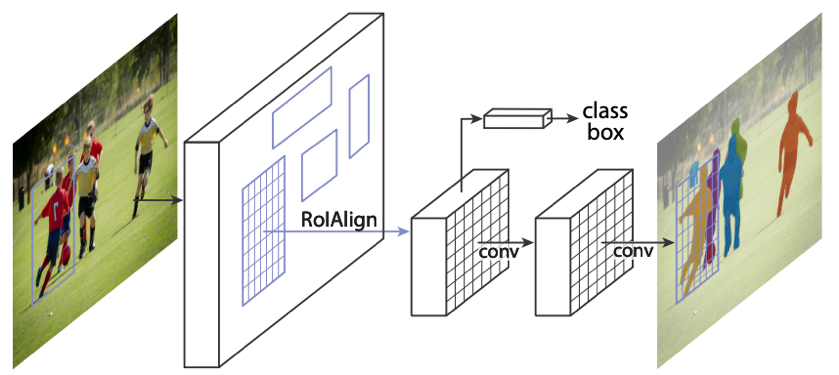
\includegraphics[width=10cm]{./figures/framework.png}
        \caption{The Mask R-CNN framework for instance segmentation.}
    \end{figure}
    \begin{figure}[htb]
		\centering
\includegraphics[width=10cm]{./figures/reslut_coco.png}
\caption{Mask R-CNN results on the COCO test set. }
    \end{figure}
\end{frame}

\end{document}
